%!TEX root = ../../main.tex

In this section, we introduce \emph{interacting particle Markov chain Monte Carlo} (\ipmcmc)~\citep{rainforth2016interacting},
a \pmcmc method based on an interacting pool of standard and conditional sequential Monte Carlo samplers. Like 
other PMCMC methods, \ipmcmc is a Markov chain Monte Carlo sampler on an extended space. In \ipmcmc we run a pool of 
\csmc and unconditional \smc algorithms as parallel processes that we refer to as nodes. After each run of this pool, 
we apply successive Gibbs updates to the indexes of the \csmc nodes, such that the indices of the \csmc nodes changes. 
Hence, the nodes from which retained particles are sampled can change from one MCMC iteration to the next, reducing
the sensitivity to path degeneracy relative to \pg 
by trading off exploration (\smc) and exploitation (\csmc) to achieve improved mixing of the Markov chains. Crucially, 
the pool provides numerous candidate indices at each Gibbs update, giving a significantly higher probability that an 
entirely new retained particle will be ``switched in'' than in non-interacting alternatives.  A high-level characterization
of \ipmcmc is given in Figure~\ref{fig:part:ipmcmc}.

We prove that \ipmcmc is a partially collapsed Gibbs sampler on the extended space containing the particle sets for all nodes. 
In the special case where \ipmcmc uses only \emph{one} \csmc node, it can in fact be seen as a non-trivial and unstudied 
instance of the $\alpha$-\smc-based \citep{whiteley2016} \pmcmc method introduced by \citet{huggins2015}. 
However, with \ipmcmc we extend this further to allow for an arbitrary number of \csmc and standard \smc algorithms 
with interaction.

The interaction between nodes requires only minimal communication; each node must report an estimate of the marginal likelihood 
and receive a new role (\smc or \csmc) for the next sweep. This means that \ipmcmc 
can be run in a distributed manner on multiple computers.  However, the advantages of \ipmcmc go far beyond
simple parallelization: our experimental evaluation shows that \ipmcmc outperforms both equivalent
non-interacting \pmcmc samplers as well as a single \pg sampler with the same number of particles run longer
to give a matching computational budget.
An implementation of iPMCMC is provided in the probabilistic programming system
\emph{Anglican}\footnote{\scriptsize \url{http://www.robots.ox.ac.uk/~fwood/anglican}} \citep{wood2014new} as we discuss in Chapter~\ref{sec:proginf:str}.  A general 
purpose toolbox for carrying out iPMCMC and other SMC / PMCMC inference in MATLAB is also provided by the custom-made \emph{probabilistic MATLAB} package.\footnote{\scriptsize \url{http://github.com/twgr/probabilistic_matlab}}

\begin{figure*}[t]
	\centering
	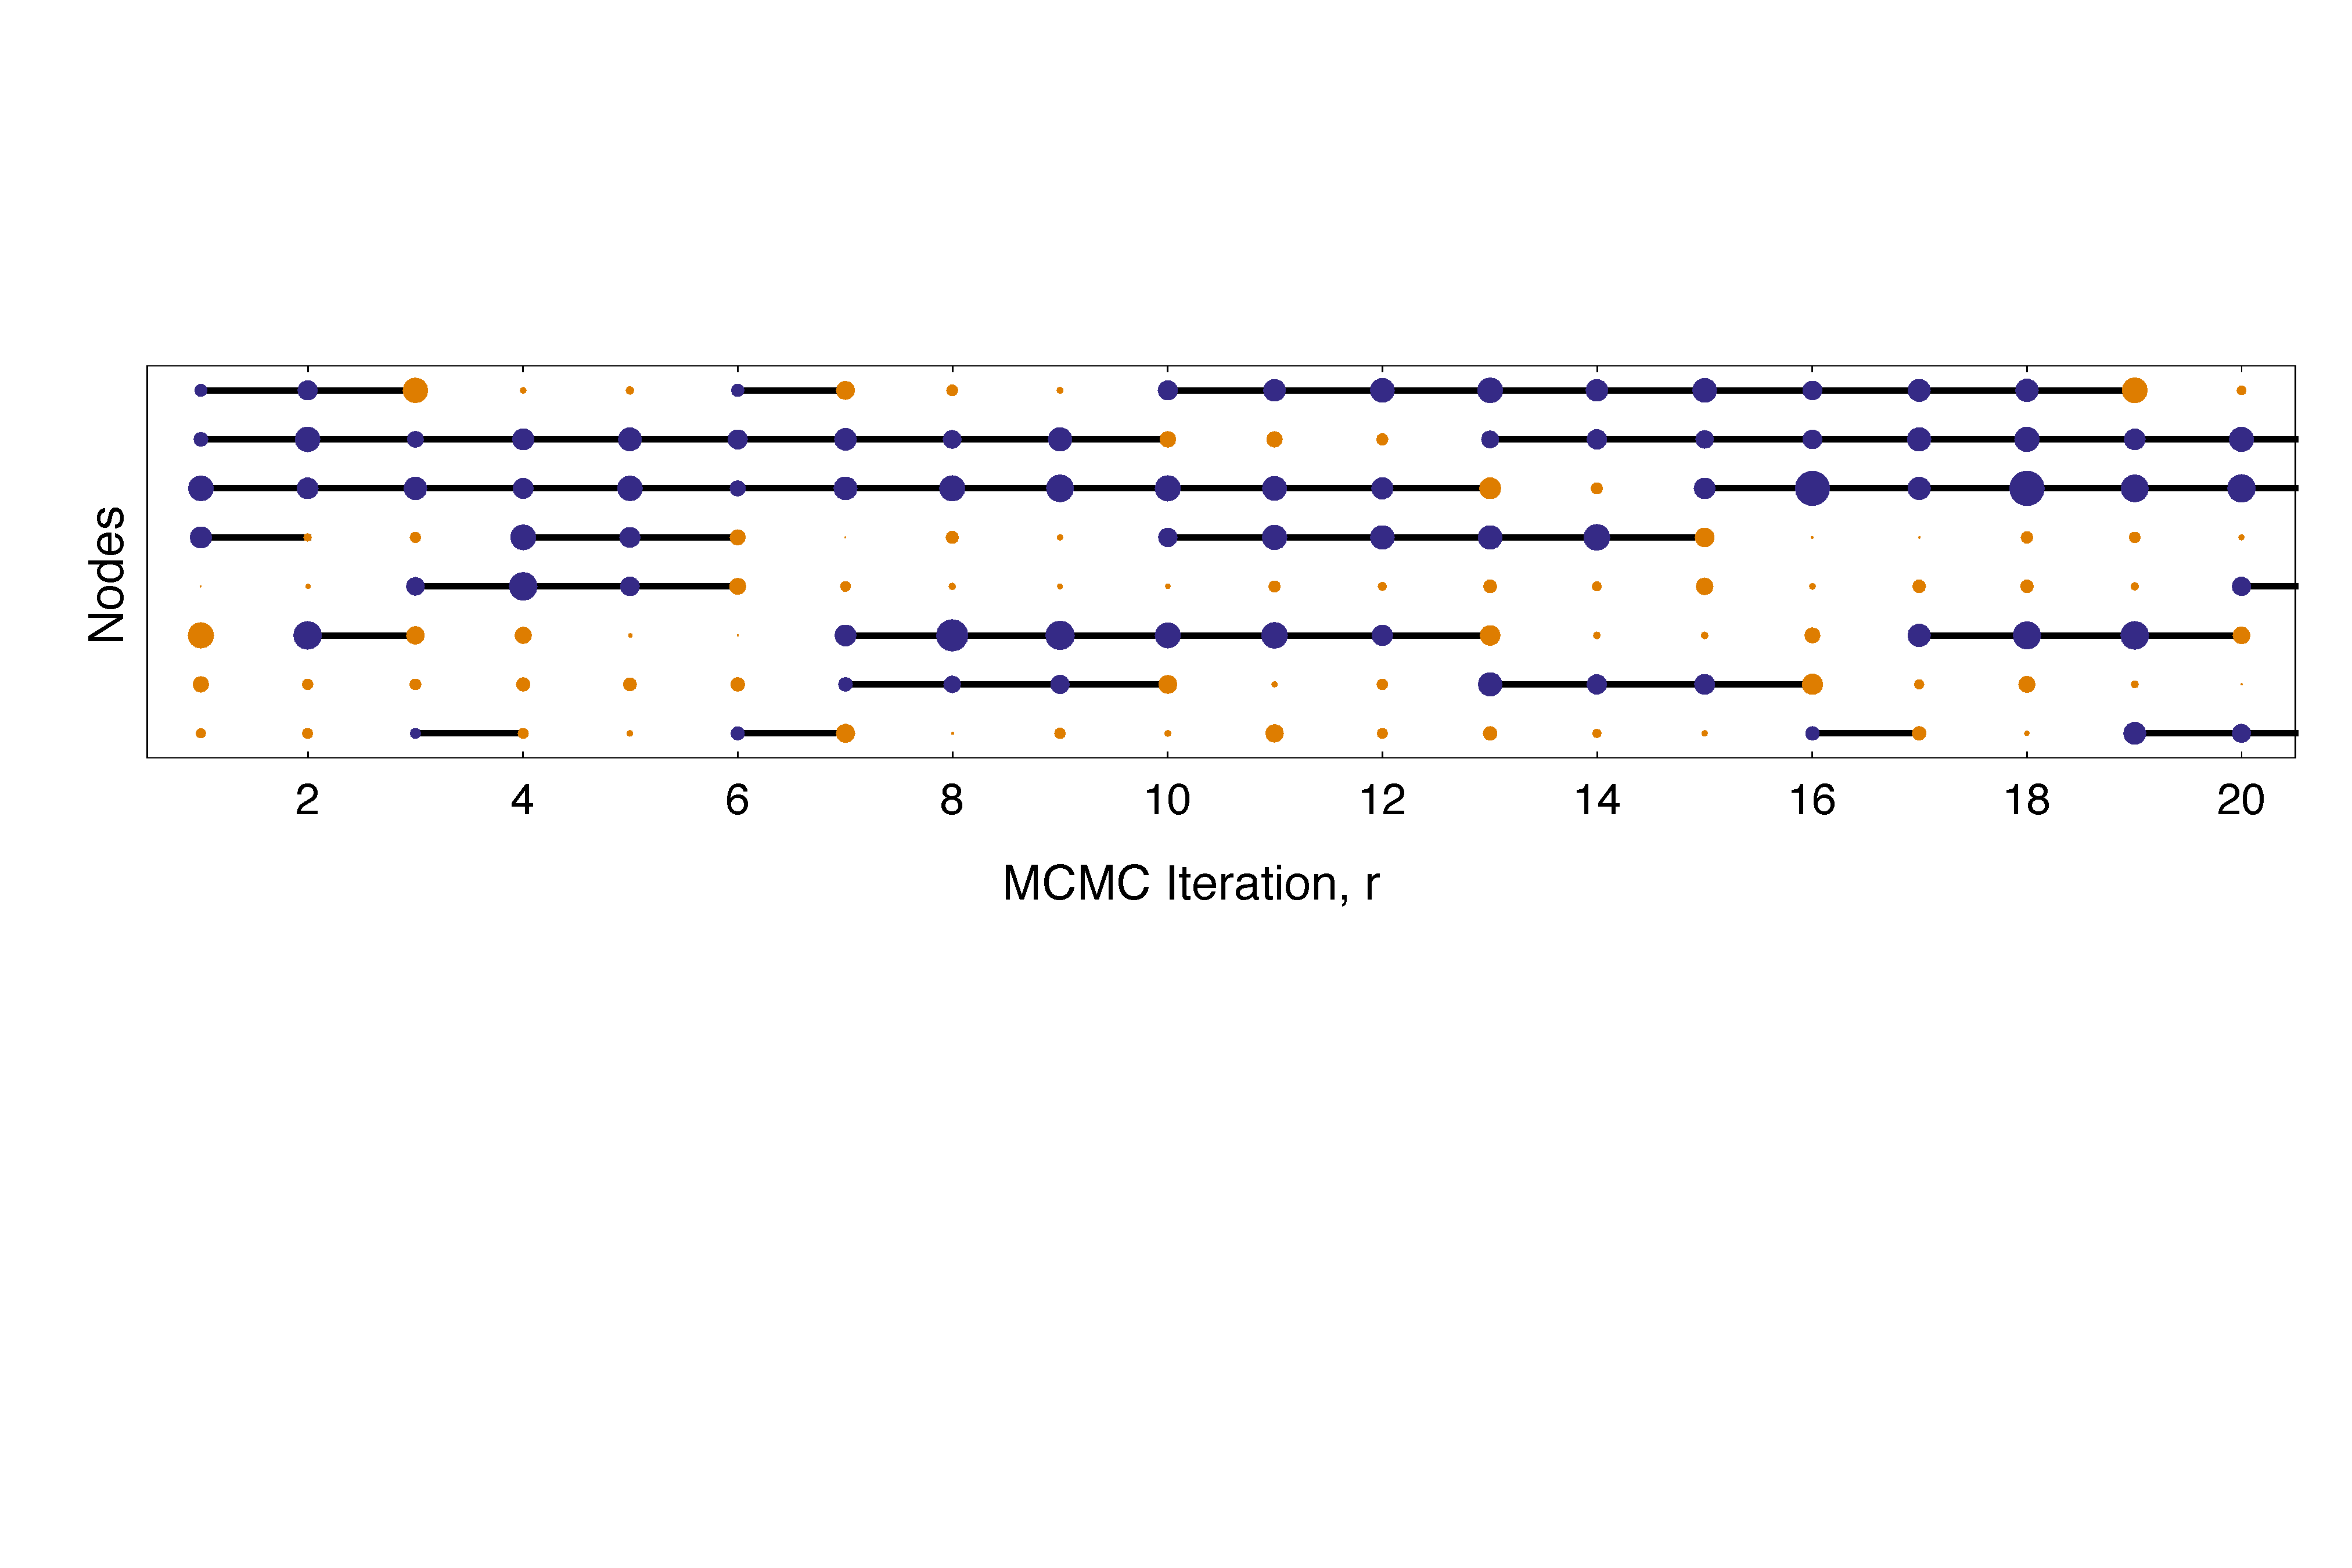
\includegraphics[width=\textwidth]{switching_example_nlss}
	\caption{Changing of conditional node indices in iPMCMC algorithm. Blue/orange nodes respectively 
		run CSMC/SMC at the next iteration. Circle sizes correspond to the
		marginal likelihood estimate produced by the sweep $\hat{Z}_m$.  Lines signify passing a retained particle. 
		We thus see that each of the nodes has breaks in the passing of retained particles, which is desirable as 
		whenever a node switches from SMC to CSMC, we must generate an entirely new retained particle. We also
		see that nodes with higher marginal likelihood estimates are more likely to become CSMC nodes at the next
		iteration.
		\label{fig:part:ipmcmc}}
\end{figure*}